\subsection{Vacuum Cleaner \cite{ai/book/Artificial-Intelligence-A-Modern-Approach/Russell-Norvig}}


\begin{figure}[H]
    \centering
    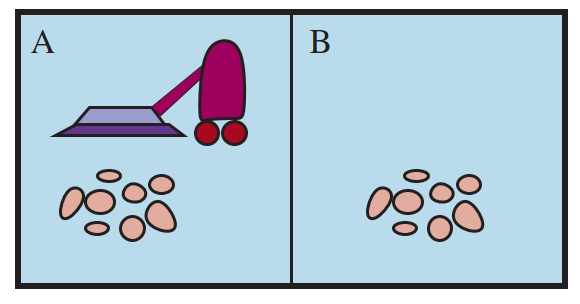
\includegraphics[
        width=0.5\linewidth
    ]{images/artificial-intelligence/examples/example-vacuum-cleaner-world.png}
    \caption*{A vacuum-cleaner world with just two locations}
\end{figure}


\vspace{0.5cm}

\begin{enumerate}[itemsep=0.2cm]
    \item it’s a made-up world

    \item This particular world has just two locations: squares A and B. 
    
    \item The vacuum agent perceives which square it is in and whether there is dirt in the square. 
    
    \item It can choose to \textbf{move left}, \textbf{move right}, \textbf{suck up the dirt}, or \textbf{do nothing}.

    \item One very simple agent function is the following: if the current square is dirty, then suck; otherwise, move to the other square.

    
\end{enumerate}



\subsubsection{As a table driven agent}

\begin{customArrayStretch}{1.3}
\begin{longtable}{|l|l|}

\hline
\textbf{Percept sequence} & \textbf{Action} \\ \hline
\endhead

\hline
\textbf{Percept sequence} & \textbf{Action} \\ \hline
\endfirsthead

\hline\endfoot
\hline\endlastfoot


$[A, \ Clean]$ & $Right$ \\ 
$[A, \ Dirty]$ & $Suck$ \\ 
$[B, \ Clean]$ & $Left$ \\ 
$[B, \ Dirty]$ & $Suck$ \\ 

\vdots & \vdots \\

$[A, \ Clean],\ [A, \ Clean]$ & $Right$ \\ 
$[A, \ Clean],\ [A, \ Dirty]$ & $Suck$ \\ 

\vdots & \vdots \\

$[A, \ Clean],\ [A, \ Clean],\ [A, \ Clean]$ & $Right$ \\ 
$[A, \ Clean],\ [A, \ Clean],\ [A, \ Dirty]$ & $Suck$ \\ 

\vdots & \vdots \\

\end{longtable}
\end{customArrayStretch}





\subsubsection{As a simple reflex agent}

\begin{algorithm}[H]
    \caption{The agent program for a simple reflex agent in the two-state vacuum environment.  \cite{ai/book/Artificial-Intelligence-A-Modern-Approach/Russell-Norvig}}

    \SetKwFunction{FUNCTION}{\textsc{Reflex-Vacuum-Agent}}
    \SetKwProg{Fn}{function}{ returns \normalfont{an action}}{end}
    \Fn{\FUNCTION{[location, status]}}{
        \textbf{if} $status \ = \ Dirty$ \textbf{then return} $Suck$ \\

        \textbf{else if} $location \ = \ A$ \textbf{then return} $Right$ \\

        \textbf{else if} $location \ = \ B$ \textbf{then return} $Left$ \\
    }
\end{algorithm}















